\documentclass[letterpaper]{article}
\usepackage[letterpaper, hmargin=0.75in, vmargin=0.75in]{geometry}
\usepackage{graphicx}
\usepackage[hyphens]{url}
\usepackage{hyperref}
\usepackage{listings}
\usepackage{pgf}
\usepackage{tikz}
\usepackage{courier}
\usepackage{amsfonts,amssymb,amsmath,amsthm,lastpage,fancyhdr,wrapfig,multirow}
\usepackage{mathrsfs}
\usepackage{palatino}
\usepackage{amsmath}
\usepackage[english]{babel}
\usepackage[utf8]{inputenc}
\usepackage{fancyhdr}
\textwidth 7.5in
\oddsidemargin -.5in
\topmargin -0.70in
\textheight 9.8in                      

\pagestyle{fancy}

%**************Fill in your ID and initials here*****************
\newcommand{\mc}[1]{\ensuremath{\mathcal{{#1}}}}
\newcommand{\mb}[1]{\ensuremath{\mathbb{{#1}}}}
\newcommand{\mf}[1]{\ensuremath{\mathfrak{{#1}}}}
\newcommand{\N}[1]{\ensuremath{\{1,\ldots,{#1}\}}}

\newcommand{\Worth}[1]{\{{#1} marks\}}
\newcommand{\Sln}{\smallskip \textbf{Solution.} }
\newcommand{\Extra}[1]{\{Extra credit: {#1} marks\}}


\setlength{\parskip}{0.15in}
\setlength{\parindent}{0in}


\newcommand{\NP}{\newpage \vspace*{-0.4in}}
\newcommand{\FP}{\vspace*{-0.6in}}
\newcommand{\tab}[1][1cm]{\hspace*{#1}}
\newcommand{\ES}{Erwin Schr\"odinger}

\lstset{ %
basicstyle=\ttfamily\scriptsize,commentstyle=\scriptsize\itshape,showstringspaces=false,breaklines=true}

\tikzstyle{input} = [coordinate]
\tikzstyle{output} = [coordinate]
\tikzstyle{joint} = [draw, circle, minimum size=1em]
\tikzstyle{block} = [draw, rectangle, minimum height=6em, minimum width=6em]


\title{\huge SE380 Notes}
\author{Minyang Jiang}
\date{\today}

\begin{document}

\maketitle

\NP
\section*{1.2 Introduction}
\subsection*{What is control engineering?}
Example (automated highway)
% \begin{center}
%   \begin{tikzpicture}[auto, node distance=2cm, >=stealth]
%     \node [input, name=input] (input) {};
%     \node [joint, right of=input] (joint1) {};
%     \node [block, right of=joint1] (controller) {Controller};
%     \node [block, right of=controller, node distance=4cm] (algorithm) {System};
%     \draw [->] (controller) -- node[name=u] {$u$} (algorithm);
%     \node [block, below of=u] (measurement) {Measurement};
%     \node [output, right of=algorithm] (output) {};

%     \draw [->] (input) -- node{$R(s)$} (joint1);
%     \draw [->] (joint1) -- node{} (controller);
%     \draw [->] (algorithm) -- node[name=y]{$Y(s)$} (output);
%     \draw [->] (y) |- node{} (measurement);
%     \draw [->] (measurement) -| node[pos=0.99]{$-$} node [near end]{$y_m$} (joint1);

%   \end{tikzpicture}
% \end{center}


Ex. web server sec1.4.1
Control Objectives
\begin{enumerate}
	\item Don't let queue length set too long
	\item Don't let queue length get to zero
\end{enumerate}
We need to keep the queue length some known value r(t)\\
the difficulty is that the \underline{service rate} is not known - depends on many things.\\
e.g. number of clients - model as a disturbances d(t)\\
We must decide on the \underline{request rate} $u(t)$ based on $r(t)$ and $y(t)$


\begin{center}
	\begin{tikzpicture}[auto, node distance=2cm, >=stealth]
		\node [input, name=input] (input) {r};
		\node [joint, right of=input] (joint1) {};
		\node [block, right of=joint1] (controller) {Controller};
		\node [joint, right of=controller] (joint2) {};
		\node [input, above of=joint2] (disturbance) {d};
		\node [block, right of=joint2, ] (server) {Server};
		\node [input, below of=joint2] (measurement) {};
		\node [output, right of=server, node distance=3cm] (output) {};
																																																										                                                                                                                                                                                                                                                                                                                                                                                                                    
		\draw [->] (input) -- node{$R(s)$} (joint1);
		\draw [->] (joint1) -- node{} (controller);
		\draw [->] (controller) -- node{} (joint2);
		\draw [->] (joint2) -- node{} (server);
		\draw [->] (disturbance) -- node [pos=0.01]{$d$} (joint2);
		\draw [->] (server) -- node[name=y]{$Y(s)$} (output);
		\draw [-] (y) |- node{} (measurement);
		\draw [->] (measurement) -| node [near end]{$y_m$} (joint1);
	\end{tikzpicture}
\end{center}

Control engineering attempts to change the behavior of a system (plant) in a useful way dispits the present of external influences (disturbances) and despite model uncertainty\\
We change the behavior of the plant by connecting it to another system (controller) Feedback is the most powerful inter-connector strategy\\
Control system
\begin{enumerate}
	\item sense the operation of system
	\item compose against a desired behavior
	\item compute a corrective action inforced by a model of the system's response to the external stimul;
	\item Actuate the system to effect demand change
\end{enumerate}
\section*{1.3 Control Engineering Design}
\begin{enumerate}
	\item Study system to be controlled; decide on sensors and actuators
	\item model resulting system
	      \begin{enumerate}
	      	\item mathematical model
	      	\item often one or more differential equations\\
	      	      e.g. follower $\frac{dx}{dt}=u$
	      \end{enumerate}
	\item Simplify model if necessary
	      Have a transfer function of the plant (input-output model)
	      e.g. follower. $$L\left \{\frac{dx_f}{dt} \right \}=L\left \{u \right\}\Rightarrow sX_f(s)=U(s)\Rightarrow\frac{X_f(s)}{U(s)}=\frac{1}{s}$$
	      a system has a TF if, and only if it is linear and time invariant
	\item Analyse resulting system
	\item Determine specifications stability, good steady behaviour robustness, good transrent performance
	\item Decide on type of controller
	\item Design controller
	      \begin{enumerate}
	      	\item in this course, the controller itself is a TF
	      	\item this TF corresponds to a diff eq relating the inputs/outputs at the controller
	      \end{enumerate}
	\item Simulate
	\item Return to step 1 if necessary
	\item Implement controller
\end{enumerate}
- the ODE from step 7 is approximated as discretized and difference equation and implemented in software\\
e.g. follower. $$u(t)=-K_p(r(kT)-y(kT)), kT\leq t\le (k+1)T$$
T: sampling period
\section*{Ch2. mathematical models of systems}

\begin{center}
	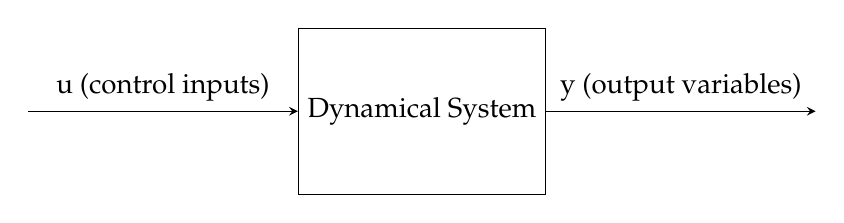
\begin{tikzpicture}[auto, node distance=2cm, >=stealth]
		\node [input, name=input] (input) {};
		\node [block, right of=input, node distance=5cm] (controller) {Dynamical System};
		\node [output, right of=controller, node distance=5cm] (output) {};
																																																										                                                                                                                                                                                                                                                                                                                                                                                                                    
		\draw [->] (input) -- node{u (control inputs)} (controller);
		\draw [->] (controller) -- node{y (output variables)} (output);
	\end{tikzpicture}
\end{center}


% \begin{center}
%   \begin{tikzpicture}[auto, node distance=2cm, >=stealth]
%     \node [block, right of=input, node distance=3cm] (b1) {Apply Known laws (Newton, queing,etc)};
%     \node [block, right of=b1, node distance=3cm] (b2) {linearize model at an operating point};
%     \node [block, right of=b2, node distance=3cm] (b3) {Take LT w/ zero initial conditions}
%     \node [block, right of=b3, node distance=3cm] (b4) {Isolate input and output}
%     \node [block, right of=b4, node distance=3cm] (b5) {Experimentally determine parameter values in TF}

%     \draw [->] (b1) -- node{System of differential equations} (b2);
%     \draw [->] (b2) -- node{System of linear differential equations} (b3);
%     \draw [->] (b3) -- node{System of linear differential equations} (b4);
%     \draw [->] (b4) -- node{Transfer Function} (b5);
%   \end{tikzpicture}
% \end{center}
\subsection*{Ex 2.1.1 mass-spring damper}
\includegraphics[scale=0.5]{images/EX2_1_1.png}
$q\in R$, position of mass M
$$q':=\frac{dq}{dt}$$
Newton's 2nd law $$Mq''=\sum \text{ forces acting on } M$$
Force due to spring $$F_k(q)=Kq \text{ assumed linear}$$
Force due to damper (possibly nonlinear) $C(q')$
$$Mq''=-Kq-C(q')+u$$
Note if the damper is linaer, i.e., $C(q')=bq$, b real constant, then the overall system is linear
\subsection*{Ex}
\includegraphics[scale=0.1]{images/EX2_1_2.jpg}\\
$u(t)$ applied voltage, $y(t)$ voltage across capacitor\\
Apply KVL 
\begin{align*}
	  & -u(t)+V_R+y=0                                   \\
	  & i_t=C\frac{dy}{dt} \text{ (capacitor equation)} \\
	  & V_R=h(i(t))=h(C\dot y)                          \\
	  & -u(t)+h(C\dot y)+y=0                            
\end{align*}
Node: If the resistor wer linear, i.e. $h(t)=R_i$ for some constant $R$, then the system is linear (Ex 2.3.4 in notes)
\subsection*{2.4 State-space models}
\subsubsection*{Ex 2.4.1}
\includegraphics[scale=0.5]{images/EX2_4_1.png}\\
Newton's 2nd law: $$M\ddot y=u-D(\dot y)$$
We put this model into a standard form by defining two so-called state variables
$$x_1:=y \text{ (position)}, x_2:=\dot y \text{ (velocity)}$$
\begin{align*}
	\dot x_1= & x_2                              \\
	\dot x_2= & \frac{1}{M}u - \frac{1}{M}D(x_2) \\
	y=        & x_1                              
\end{align*}
This is called state-space model, first two equations are called state equations, last one is called output equation.\\
These equations have the general form: $$\dot x=f(x,u)$$ $$y=h(x)$$ where (in this example ) $$x=(x_1,x_2)\in R^2$$ $$f(x,u)=\begin{bmatrix}x_2\\ \frac{1}{M}u-\frac{1}{M}D(x_2)\end{bmatrix}, h(x)=x_1$$
In the special case, where air resistance is a linear function of $x_2:D(x_2)=dx_2$, d real constant, then $f(x,u)$ becomes a linear function of $x$ and $u$
$$f(x,u)=
\begin{bmatrix} 
	0 & 1 \\0&\frac{-d}{M}
\end{bmatrix} 
\begin{bmatrix} 
	x_1 \\x_2
\end{bmatrix} +
\begin{bmatrix} 
	0 \\\frac{1}{M}
\end{bmatrix}
u$$
Define 
$C:= 
\begin{bmatrix}
	1 & 0 
\end{bmatrix}$
we get 
\begin{align*}
	\dot x= & Ax+Bu \\
	y=      & Cx    
\end{align*}

Generalizing Ex 2.4.1, an important class of systems have models of the form:
\begin{align*}
	\dot x= & f(x,u),f: \mathbb{R}^n*\mathbb{R}^m\rightarrow \mathbb{R}^n \\
	\dot y= & h(x,u), h:\mathbb{R}^n*\mathbb{R}^m\rightarrow \mathbb{R}^p 
\end{align*}
- this model is nonlinear.\\
- there are m control inputs, $u=(u_1,u_2,\hdots, u_m)$\\
- there are p outputs $y=(y_1,y_2,\hdots,y_p)$\\
- the state vector x has dimension n: $x=(x_1,\hdots,x_n)$\\

e.g.\\
\includegraphics[scale=0.8]{images/Figure_2_30.png}\\
$m=2, u=(u_1,u_2)$\\
$p=2, y=(y_1,y_2)$\\
$n=4, x=(x_1,x_2,x_3,x_4):=(y_1,\dot y_1, y2, \dot y_2)$

\underline{Ex (Quarotor UAV)}\\
$m=4, u=(u_1,u_2,u_3,u_4)=(f_1,f_2,f_3,f_4)$\\
$p=3,y=(y_1,y_2,y_3)$\\
$x\in \mathbb R^{12}=(\text{position, orientation, velocity, angular velocity})$

-The linear special case is:
\begin{align*}
	\dot x= & Ax+Bu, A\in \mathbb{R}^{n*n},B\in \mathbb{R}^{n*m}  \\
	y=      & Cx+Du, C\in \mathbb{R}^{p*n}, D\in \mathbb{R}^{p*m} \\
\end{align*}

- In this course, single input-output systems $$m=p=1$$
What is the state of a system? \\
The state vector $x(t_0)$ encapsulates all of the systems dynamics up to time $t_0$

More formally: for any two times $t_0<t_1$, knowing $x(t_0)$ and knowing $\{u(t): t_0 \leq t\leq t_1\}$, we can compute $x(t_1)$ and $y(t_1)$

\subsubsection*{Ex 2.4.2}
No force on system $$M\ddot y=0$$
If we try a 1-dimensional state, say $x:=y$, then knowing $x(t_0)$ without knowing $\dot y(t_0)$, we cannot compute $x(t)$ for $t>t_0$\\
Same problem with $x:=\dot y$\\
- Since the governing equation is $2^{nd}$ order we need two initial conditions, So $x=(y,\dot y)\in \mathbb{R}^2$ is a good choice.

\subsubsection*{Ex 2.5.1}
\includegraphics[scale=0.9]{images/Ex2_5_1.png}\\
Model (see Ex 2.3.3) is 
$$\ddot \Theta = \frac{3}{Ml^2}u-3\frac{g}{l}\sin(\Theta)$$
To put this system in state-space form\\
\begin{enumerate}
	\item[1)] $x:=(\Theta, \dot \Theta)$
	\item[2)] $y=$angular position=$\Theta$
\end{enumerate}
\begin{align*}
	\dot x_1= & x_2                                   \\
	\dot x_2= & \frac{3}{Ml^2}u-\frac{3g}{l}\sin(x_1) 
\end{align*}


\subsubsection*{Ex 2.4.5}
\includegraphics[scale=0.9]{images/Ex2_4_5.png}\\
choose: $$x_1:=\text{voltage across cap}=\frac{1}{C}\int y(\tau)d\tau$$
$$x_2:=\text{current through inductor}=y$$
KVL:
\begin{align*}
	  & -u+V_R+V_C+V_L=0\Rightarrow-u+Rx_2+x_1+L\dot x_2=0 \\
	  & \dot x_1=\frac{1}{C}x_2                            
\end{align*}
\begin{align*}
	\dot x=&
	\begin{bmatrix}
	0&\frac{1}{C}\\
	\frac{-1}{L}&\frac{-R}{L}
	\end{bmatrix}
	\begin{bmatrix}
	x_1\\x_2
	\end{bmatrix}
	+\begin{bmatrix}
	0\\\frac{1}{L}
	\end{bmatrix}u\\
	y= & \begin{bmatrix} 0 & 1\end{bmatrix}x 
\end{align*}

\subsection*{2.5 Linearization}
- linearization - approximate a nonlinear state-space model with a linear one.\\
- linearization allows us to use simple systematic design methods\\
\subsubsection{Ex 2.5.2}
Linearize $y=x^3$ at the point $\bar x=1$\\
Taylor series at $x=\bar x$ is $$y=\sum_{n=0}^{\infty} c_n(x-\bar x)^n,c_n=\frac{d^nf(x)}{dx^n}\vert_{x=\bar x}* \frac{1}{n!}$$
- keep only the terms $n=0,n=1$, $$f(x)\approx f(\bar x)+\frac{df(x)}{dx}(x-\bar x)$$
$$y-\bar y\approx \frac{df}{dx}\vert_{x=\bar x}(x-\bar x)$$
If we define the deviations $\partial y:=y-\bar y, \partial x:=x-\bar x$, then $$\partial y=\frac{df}{dx}\vert_{x=\bar x}*\partial x$$ 

\subsubsection*{Ex 2.5.3}
\begin{align*}
	y=\begin{bmatrix} y_1 \\y_2\end{bmatrix}=f(x)=\begin{bmatrix}x_1x_2-1\\x_3^2-2x_1x_3\end{bmatrix}=\begin{bmatrix} f_1(x)\\f_2(x)\end{bmatrix}
\end{align*}

\begin{align*}
	\bar y=f(\bar x)=\begin{bmatrix}-2 \\0\end{bmatrix}
\end{align*}
- multivariable Taylors: $$f(x)=f(\bar x)+\frac{\partial f}{\partial x}\vert_x=\bar x*(x-\bar x)+\text{ higher order terms}$$
\begin{align*}
	\frac{\partial f}{\partial x}\vert_{x=\bar x}=&\text{ Jacobian of f evaluated at }x=\bar x\\
	=&\begin{bmatrix}
	\frac{\partial f_1}{\partial x_1} & \frac{\partial f_1}{\partial x_2} & \frac{\partial f_1}{\partial x_3} \\
	\frac{\partial f_2}{\partial x_1} & \frac{\partial f_2}{\partial x_2} & \frac{\partial f_2}{\partial x_3} \\
	\end{bmatrix}_{x=\bar x}\\
	=&\begin{bmatrix}
	x_2                               & x_1                               & 0                                 \\
	-2x_3                             & 0                                 & 2x_3-2x_1                         
	\end{bmatrix}_{x=(1,2,3)}\\
	=&\begin{bmatrix}
	-1                                & 1                                 & 0                                 \\
	-4                                & 0                                 & 2                                 
	\end{bmatrix}=: A
\end{align*}
- by direct extension : $$f(x,u)\approx f(\bar x, \bar u)+\frac{\partial f}{\partial x}\vert_{(x,u)=(\bar x,\bar u)}(x-\bar x)+\frac{\partial f}{\partial u}\vert_{(x,u)=(\bar x,\bar u)}(u-\bar u)$$
- Let's apply this to 
\begin{align*}
	\dot x= & f(x,u) \\
	y=      & (x,u)  
\end{align*}
\subsubsection*{DEFN 2.5.1} A constant pair $(\bar x, \bar u)\in \mathbb{R}^n*\mathbb{R}^n$ is an equilibrium configuration of (*) if $f(\bar x, \bar u)=(0,0,0,0,\hdots,0)$\\
The constant $\bar x$ is the equilibrium point
\subsubsection*{\underline{Ex}}
Find all equilibrium at which the pendulum is upright\\
$\dot x=f(x,u),y=h(x,u)$\\
$f(x,u)=\begin{bmatrix}x_2\\\frac{3}{Ml}u-\frac{3g}{l}\sin(x_1)\end{bmatrix},h(x)=x_1$\\
$x_1=\Theta, x_2=\dot\\ \Theta$\\
If $y=\Pi$ then $\bar x_1=\Pi$ So we have to solve $$\begin{bmatrix}0\\0\end{bmatrix}=\begin{bmatrix}x_2\\\frac{3}{Ml}u-\frac{3g}{l}\sin(x_1)\end{bmatrix}\Rightarrow \bar x_2=0, \bar u=0$$
  
Conclusion: the equilibrium are $$\begin{bmatrix}\bar x_1\\\bar x_2\end{bmatrix}=\begin{bmatrix}\Pi+2\Pi k\\0\end{bmatrix}, \bar u=0, k\in \mathbb{Z}$$
Assume $\dot x=f(x,u)$ has an eq config at $(x,u)=(\bar x, \bar u)$
$$f(x,u)\approx f(\bar x,\bar u)+\frac{\partial f}{\partial x}\vert_{(x,u)=(\bar x,\bar u)}(x-\bar x)+\frac{\partial f}{\partial u}\vert_{(x,u)=(\bar x,\bar u)}(u-\bar u)=0+A\partial x + B \partial u$$
- consider deviatiors from $(\bar x,\bar u)$ $$\partial x(t)=x(t)-\bar x$$ $$\partial u(t)=u(t)-\bar u$$
- Then $$\dot \partial x=\dot x -0=f(x,u)\approx A\partial x + B \partial u$$
i.e. \begin{equation}
\dot \partial x=A\partial x+B\partial u \text{ linearized state equation}
\end{equation}
- linearized output equations: $$\partial y=\frac{\partial h}{\partial x}\vert_{(x,u)=(\bar x,\bar u)}\partial x+\frac{\partial h}{\partial u}\vert_{(x,u)=(\bar x,\bar u)}\partial u=C\partial x+D\partial u$$
Summary: Linearizing $\dot x=f(x,u), y=h(x,u)$
\begin{enumerate}
	\item select an eq. config $(\bar x,\bar u)\in \mathbb{R}^n*\mathbb{R}^m$ $$\bar y=(\bar x,\bar u), f(\bar x,\bar u)=0$$
	\item Compute Jacobians of f, h to get A,B,C,D
	\item Linearization: $$\dot \partial x=A\partial x+B\partial u$$ $$\partial y=C\partial x+D\partial u$$
\end{enumerate}
\subsubsection*{Ex 2.5.4}
Linearize pendulum at upright position
\begin{align*}
	\dot x_1= & x_2                                 \\
	\dot x_2= & \frac{3}{Ml}u-\frac{3g}{l}\sin{x_1} \\
	y=        & x_1                                 
\end{align*}
\begin{enumerate}
	\item The eq. config at the upright position is $(\bar x, \bar u)=(
	      \begin{bmatrix}\pi\\0\end{bmatrix}, 0)$
	\item $A=\begin{bmatrix} 0&&1\\ \frac{-3g\cos{x_1}}{l}&&0\end{bmatrix}=\begin{bmatrix}0&&1\\ \frac{3g}{l}&&0\end{bmatrix}$\\
	      $B=\begin{bmatrix}0\\\frac{3}{Ml}\end{bmatrix}$\\
	      $C=\begin{bmatrix} 1&& 0\end{bmatrix}$\\
	      $D=0$
	\item
	      \begin{align*}
	      	\dot \delta x= & \begin{bmatrix} 0 &   & 1 \\\frac{3g}{l}&&0\end{bmatrix}\delta x+\begin{bmatrix} 0\\\frac{3}{Ml}\end{bmatrix}\delta u\\
	      	\delta y=& \begin{bmatrix}1&& 0\end{bmatrix}\delta x+\begin{bmatrix}0\end{bmatrix}\delta u\\
	      	\delta x(t)=&x(t)-\begin{bmatrix}\pi\\0\end{bmatrix}\\
	      	\delta u(t)=&u(t)-0
	      \end{align*}    	
\end{enumerate}
		    
\begin{center}
	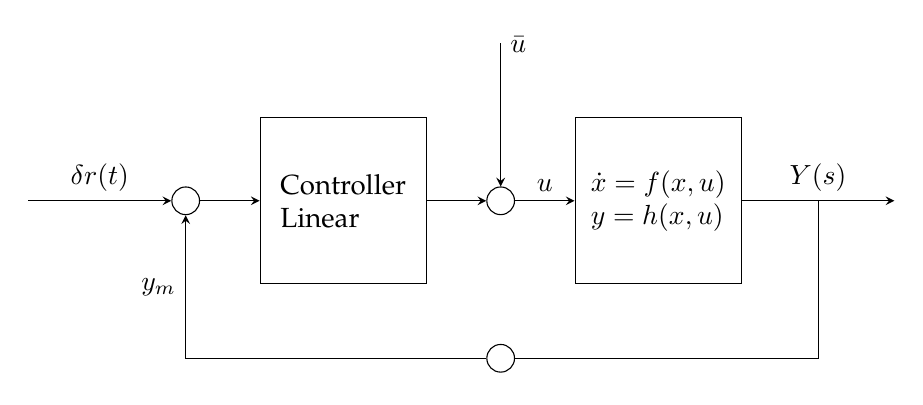
\begin{tikzpicture}[auto, node distance=2cm, >=stealth]
		\node [input, name=input] (input) {r};
		\node [joint, right of=input] (joint1) {};
		\node [block, right of=joint1, align=left] (controller) {Controller\\Linear};
		\node [joint, right of=controller] (joint2) {};
		\node [input, above of=joint2] (disturbance) {d};
		\node [block, right of=joint2, align=left] (server) {$\dot x=f(x,u)$\\$y=h(x,u)$};
		\node [joint, below of=joint2] (measurement) {};
		\node [output, right of=server, node distance=3cm] (output) {};
																																																										                                                                                                                                                                                                                                                                                                                                                                                                                    
		\draw [->] (input) -- node{$\delta r(t)$} (joint1);
		\draw [->] (joint1) -- node{} (controller);
		\draw [->] (controller) -- node{} (joint2);
		\draw [->] (joint2) -- node{$u$} (server);
		\draw [->] (disturbance) -- node [pos=0.01]{$\bar u$} (joint2);
		\draw [->] (server) -- node[name=y]{$Y(s)$} (output);
		\draw [-] (y) |- node{} (measurement);
		\draw [->] (measurement) -| node [near end]{$y_m$} (joint1);
	\end{tikzpicture}
\end{center}		    
		    
		    
\section*{2.8 Transfer Functions}
\begin{enumerate}
	\item LTI system, and only LTI systems, have transfer functions
	\item it is the ratio $\frac{Y(s)}{U(s)}$ where $Y(s)=L\{y(t)\},u(s)=L\{u(t)\}$ and the LTs are taken with zero initial conditions
\end{enumerate}	
\subsubsection*{Ex 2.8.3}
Mass-spring-dumper $$M\ddot q=u-Kq -c(\dot q)$$	    
Take $y:=q$ as system output, if $c(\dot q)$ is a nonlinear function, there is no TF.\\
if $c(\dot q)=b\dot q, b\in \mathbb{R}$ then
\begin{align*}
	            & s^2MQ(s)=U(s)-KQ(s)-sbQ(s)\text{ zero initial conditions} \\
	\Rightarrow & \frac{Q(s)}{U(s)}=\frac{1}{s^2M+sb+K}                     
\end{align*}
Other examples (Table 2.2)
\subsubsection*{DEFN 2.8.1} A TF $G(s)$ is real rational
\begin{enumerate}
	\item $$G(s)=\frac{b_ms^m+\hdots+b_1s+b_0}{s^n+a_{n-1}s^{n-1}+\hdots+a_1s+s_0},a_i,b_i\in \mathbb{R}$$
	      Let $\mathbb{R}(s)$ be the set of all real rational TFs
	\item $G(s)\in \mathbb{R}(s)$ is proper if $n\geq m$
	\item $G(s) \in \mathbb{R}(s)$ is strictly proper if $n > m$
\end{enumerate}
\subsubsection*{DEFN 2.8.2}
A complex number $p\in \mathbb{C}$ is a pole of $G(s)$ if $\lim_{s\rightarrow p}|G(s)|=\infty$
If $G(s)\in \mathbb{R}(s)$ and its numerator and denominator are co-prime then poles of G=roots of denom, zeros of G=roots of numerator		    
		    
\subsection*{2.8.1 state-space to transfer function}
start with $$\dot x=Ax+Bu$$$$y=Cx+Du$$
take LTs with zero initial conditions
\begin{align*}
	sX(s)= & AX(s)+BU(s)           \\
	Y(s)=  & CX(s)+DU(s)           \\
	X(s)=  & (X_1(s)\hdots,X_n(s)) \\
	U(s)=  & (U_1(s)\hdots,U_m(s)) \\
	Y(s)=  & (Y_1(s)\hdots,Y_p(s)) \\
\end{align*}	    

eliminate $X(s)$
\begin{align*}
	            & (sI-A)X(s)=BU(s)                \\
	\Rightarrow & X(s)=(sI-A)^{-1}BU(s)           \\
	\Rightarrow & Y(s)=[C(sI-A)^{-1}B+D]U(s)=G(s) 
\end{align*}
Remark 2.8.3 - the TF obtained from a state-space model is always rational and always proper.\\
state-space model $\Rightarrow$ rational proper TF function\\
TF model $\Rightarrow$ state-space model (only when TF is rational and proper, answer is never unique)
\subsubsection*{Ex 2.8.6} Linearized pendulum at $\bar x=\begin{bmatrix}\pi\\0\end{bmatrix},\bar u=0$

\section*{Sommary Lecture \#8}
\begin{enumerate}
	\item $$\dot x=Ax,x(0)=x_0\in\mathbb{R}^n$$
	      solution is $x(t)=e^{At}x_0$\\
	      $e^{At}=$matrix exponential $=I+tA+\frac{t^2A^2}{2!}+\hdots=\mathbb{L}^{-1}\{(sI-A)^{-1}\}$
	\item $\dot x=A+Bu,x(0)=x_0,u(t)=a$,"resonable" input\\
	      solution $$x(t)=e^{At}x_0+\int_0^t e^{A(t-\tau)}Bu(\tau)d\tau=\text{initial state response + forced response}$$
	\item $\dot x=Ax$ is asymptotically stable if $x(t)\rightarrow 0$ for any $x(0)$ all eigenvalue of A have negative real part
\end{enumerate}

\section*{3.5 bounded input bounded output stability}
$$y(t)=(g*u)(t),y=L^{-1}\{G\}$$
\subsection*{DEFN 3.5.2} An LTI system in BIBO stable, if every  bounded input produces a bounded output $$\|u\|_\infty \text{ finite }\Rightarrow \|y\|_\infty \text{ finite}_o$$
\subsection*{Ex 3.5.1}
$G(s)=\frac{1}{s+2}$, Impulse response $g(t)=\mathscr{L}^{-1}\{G(s)\}=e^{-2t}$
\begin{align*}
	y(t)= & (g*u)(t)                         \\
	=     & \int_0^te^{-2\tau}u(t-\tau)d\tau 
\end{align*}
So, for all $t\geq 0$
\begin{align*}
	|y(t)|= & \lvert \int_0^te^{-2\tau}u(t-\tau)d\tau\rvert                            \\
	\leq    & \int_0^t\lvert e^{-2\tau}u(t-\tau)\rvert d\tau                           \\
	\leq    & \int_0^te^{-2\tau}d\tau \|u\|_{\infty}                                   \\
	\leq    & \int_0^{\infty}e^{-2\tau}d\tau \|u\|_{\infty} =\frac{1}{2}\|u\|_{\infty} 
\end{align*}
Conclusion: $$\|y\|_{\infty}\leq \frac{1}{2}\|u\|_{\infty}$$
So system is BIBO stable.
\subsection*{THM 3.5.3} Assume $G(s)$ is rational and strictly proper. Then the following are equivalent:
\begin{enumerate}
	\item G is BIBO stable
	\item impulse response $g(t)=\mathscr{L}^{-1}\{G(s)\}$is absolutely integrable
	      $$\int_0^{\infty}|g(\tau|d\tau<\infty$$
	\item Every pole of G has negative real part.
	      e.g. $$\frac{1}{s+1},\frac{1}{(s+3)^2},\frac{s-1}{s^2+5s+6}\text{ BIBO stable}$$
	      $$\frac{1}{s},\frac{1}{s-1} \text{ BIBO unstable}$$
\end{enumerate}
\subsection*{THM 3.5.5} If G(s) is rational and improper, the G is not BIBO stable.\\
Proof: Using long division, write $G(s)=G_1(s)+G_2(s)$, $G_1$ - strictly proper, $G_2$ polynomial in s.\\
e.g. $G(s)=\frac{s^2+1}{s}$ then $G_s(s)=s$and $G_1(s)=\frac{1}{s}$\\
use linearity to write $Y(s)=G_1(s)U(s)+G_2(s)U(s)$\\
- if $G_1$ has poles in $Re(s)\geq 0$ then result follows from THM 3.5.4\\
- if $G_1$ has all poles in $Re(s) < 0$\\
Then choose $u(t)=\sin(t^2)$\\
- then $Y_1$ is bounded by THM 3.5.4\\
- any derivative of u has polynomial terms in t, so derivative is not bounded\\
- But $y_2$ is a linear combo of u and its time derivatives, so $y_2$ is not bounded.
\subsubsection*{3.5.1} Stability of state space models and BIBO stability\\
\begin{align*}
	\dot x= & Ax+Bu \\
	y=      & Cx+Du 
\end{align*}

\begin{align*}
	Y(s)= & [C(sI-A)^{-1}B+D]U(s)                      \\
	=     & [C\frac{adj(sI-A)}{det(sI-A)}B+D]U(s)      \\
	      & \text{BIBO stable if all poles in }Re(s)<0 
\end{align*}
Asymptotically stable if all eigenvalues of A in $Re(s)<0$\\
eigenvalue of $A=\text{roots of det}(sI-A)\supseteq \text{poles of }G(s)=C(sI-A)^{-1}B+D$\\
usually $C adj(sI-A)B$ and $det(sI-A)$ are co-prime	\\
In whichi case the two notions are equivalent.
\subsection*{Ex 3.5.5} (mass-spring)
\begin{align*}
	\dot x= & \begin{bmatrix}0 & 1 \\-4&0\end{bmatrix}x+\begin{bmatrix}0\\1\end{bmatrix}u\\
	y=&\begin{bmatrix}1&0\end{bmatrix}x\\
	\frac{Y(s)}{U(s)}=&\frac{1}{s^2+4}=G(s)
\end{align*}
System is not BIBO stable
so eigenvalue of A = poles of G

\section*{Summary Lecture \#9}		    
- DEFN of BIBO stability (I.O. notion)\\
- checking BIBO stability \\
\begin{enumerate}
	\item all poles of TF in $\mathbb{C}$
	\item $\int_{0}^t |g(\tau)|d\tau < \infty, g=\mathscr{L}^{-1}\{G\}$ 
\end{enumerate}
- G improper $\Rightarrow$ BIBO stable\\
- Asymptotic stability $\Rightarrow$ BIBO stability\\

\section*{3.6 Steady-state gain}
steady-state gain of G(s) is $\frac{y_{ss}}{b}$, b is input\\
\subsection*{THM 3.6.1} (Final Value Theorem)
$$F(s)=\mathscr{L}\{f(t\}, \text{ assume F(s) is rational}$$
\begin{enumerate}
	\item if $F(s)$ has all poles in $Re(s)<0$, then $\lim_{t\rightarrow \infty} f(t)=0$\\
	      e.g. $$F(s)=\frac{1}{s+1},f(t)=e^{-t}$$ 
	\item if $sF(s)$ has all poles in $Re(s) < 0$, then $$\lim_{t\rightarrow \infty}f(t)=\lim_{x\rightarrow 0} sF(s)$$
	\item if $sF(s)$ has even one pole with $Re(s) \geq 0$, then $f(t)$ does not converge.\\ e.g. $$F(s)=\frac{1}{s^2}, sF(s)=\frac{1}{s},f(t)=t$$
\end{enumerate}
Example\\
\begin{center}
	\begin{tabular}{ l | c | c | c | r }
		\hline
		f(t)            & $\lim_{t\rightarrow \infty} f(t)$ & $F(s)$                   & $\lim_{s\rightarrow 0}sF(s)$ & FVT case \\ \hline
		$e^{-t}$        & 0                                 & $\frac{1}{s+1}$          & 0                            & 1 or 2   \\ \hline
		$1(t)$          & 1                                 & $\frac{1}{s}$            & 1                            & 2        \\ \hline 
		t               & $\infty$                          & $\frac{1}{s^2}$          & $\infty$                     & 3        \\ \hline 
		$te^{-t}$       & 0                                 & $\frac{1}{(s+1)^2}$      & 0                            & 1 or 2   \\ \hline 
		$e^t$           & $\infty$                          & $\frac{1}{s-1}$          & 0                            & 2        \\ \hline 
		$\cos(\omega t)$ & N/A                               & $\frac{s}{s^2+\omega^2}$ & 0                            & 3        \\ 
		\hline
	\end{tabular}
\end{center}
\subsection*{THM 3.6.2}
If $G(s)$ is BIBO stable and $u(t)=b1(t)$, then $y_{ss}=bG(0)$. Invite you to prove it via Final value Theorem.\\
i.e. steady state gain is always $\frac{y_{ss}}{b}=G(0)$ for and b!\\
Example (set-point control)
\begin{align*}
\dot x=&-2x+u\\
y=&x\\
\Rightarrow Y(s)=&\frac{1}{s+2}U(s)
\end{align*}		    
Problem: Given a constant reference $r(t)=r_01(t), r_0$ constant, find a control signal $u(t)$ to make $y(t)\rightarrow r(t)$ as $t\rightarrow \infty$\\
We want $$\lim_{t\rightarrow \infty} y(t)=r_0$$
\begin{align*}
y_{ss}=\lim_{t\rightarrow \infty} y(t) &=\lim_{s\rightarrow 0} sC(s)P(s)R(s)\\
&=\lim_{s\rightarrow 0}sC(s)\frac{1}{s+2}\frac{r_0}{s}
\end{align*}
If $C(s0$ is BIBO stable, then $y_{ss}=\lim_{s\rightarrow 0} C(s)\frac{1}{s+2}r_0=C(0)\frac{1}{2}r_0$: $$y_{ss}=r_0 \iff C(0)=2=\frac{1}{P(0)}$$
Simplest choice: $$C(s)=\frac{1}{P(0)}=2$$
\subsection*{3.7 Frequency Response}
$Y(s) = G(s)U(s)$ or $y(t)=(g*u)(t)$
\subsection*{THM 3.7.1}
Assume G ration, BIBO stable. If $u(t)=\cos(\omega t)$, then the steady state output is: 
$$y(t)=A\cos(\omega t+\phi), A=|G(j\omega)|,\phi=\angle G(j\omega)$$
\subsection*{Ex}
\begin{align*}
\dot x=&-10x+u\\
y=&x\\
\Rightarrow Y(s)=&\frac{1}{s+10}U(s)=G(s)U(s)\\
A=&-10\\
det(sI-A)=s&+10\\
&\text{eigenvalue of A is -10}
\end{align*}
If $u(t)=2\cos(3t+\frac{\pi}{6})$, what is the steady-state output?
System is asymptotically stable $\Rightarrow$ BIBO stable $\Rightarrow$ THM 3.7.1 applies\\
From THM 3.7.1 steady-state output is $y(t)=2A\cos(3t+\frac{\pi}{6}+\phi)$\\
$A=|G(j\omega)|=|G(j3)|=|\frac{1}{j3+10}|=\frac{1}{\sqrt{3^2+10^2}}\approx 0.1$\
$\phi=\angle G(j3)=\angle \frac{1}{j3+10}=\angle 1-\angle (j3+10)=-arctan(10,3)\in (-\pi,\pi]$

\subsection*{DEFN 3.7.2}
If $G(s) \in \mathbb{R}(s)$ and BIBO stable
\begin{enumerate}
	\item the function $\mathbb{R} \rightarrow \mathbb{C}, \omega\rightarrow G(j\omega)$ is the frequency response.
	\item the function $\mathbb{R} \rightarrow \mathbb{R},\omega\rightarrow|G(j\omega)|$ is the magnitude response.
	\item the function $\mathbb{R}\rightarrow (-\pi,\pi], \omega \rightarrow \angle G(j\omega)$ is the phase response.
\end{enumerate}

\section{Grophical Representations of frequency response}
when we graph $G(j\omega)$ we only consider $\omega \geq 0$, no loss of info when G is rational $|G(j\omega)|=|G(-j\omega)|, \angle G(j\omega)=-\angle G(-j\omega)$\\
Bode Plots
\begin{enumerate}
	\item magitude plot: $20log|G(j\omega)|$ vs $log(\omega)$
	\item phase $\angle G(j\omega)$ vs $og(\omega)$	
\end{enumerate}
Polar Plots: $Re(G(j\omega))$ vs $\ln(G(j\omega))$\\
- to sketch the Bode plot of any rational TF, we only need to know how to sketch 4 terms.
\begin{enumerate}
	\item Pure gain $G(s)=K$
	\item first order $G(s)=\tau s \pm 1,\tau > 0$
	\item Zeros at s=0 $G(s)=s^n$
	\item complex conjugate roots $$G(s)=s^2+2z\omega_ns+\omega_n^2$$
\end{enumerate}
\subsection*{Ex 3.8.5}
\begin{align*}
G(s)=&\frac{40s^2(s-2)}{(s+5)(s^2+4s+100)}\\
=&\frac{(40)s^2(2)(\frac{s}{2}-1))}{(5)(100)(\frac{s}{5}+1)(\frac{s^2}{10^2}+\frac{4s}{10^2}+1)}\\
=&\frac{(40)(2)}{(5)(100)}\frac{s^2}{\frac{s}{5}+1}\frac{\frac{s}{2}-1}{\frac{s^2}{10^2}+\frac{4s}{10^2}+1}
\end{align*}
\subsection*{Ex 3.8.6 To plot Bode plot we need}
\begin{align*}
20log|G(j\omega)|=20log|\frac{80}{500}|+20log|(j\omega^2)|-20log|\frac{j\omega}{2}-1|-20log|\frac{j\omega}{5}+1|-20log|\frac{(j\omega)^2}{10^2}+\frac{4}{10^2}j\omega + 1|
\end{align*}
\begin{enumerate}
	\item $G(s)=K$
	\item $G(j\omega)j\tau\omega+1$ (TF with a zero at $s=\frac{-1}{\tau}$)\\
	Bode plot $$20log|G(j\omega)|=20log|j\omega \tau +1|$$
	Approximates for sketching
	\begin{enumerate}
		\item for $\omega < \frac{1}{\tau}$, $Im(G(j\omega)) \approx 0\Rightarrow (\forall \omega < \frac{1}{\tau})20log|G(j\omega)|\approx 2 log|1|=0$
	\end{enumerate}
	\end{enumerate}

































































\end{document}